\documentclass[11pt]{article}
\usepackage{tikz}
\usetikzlibrary{scopes}
\usepackage{amsmath}
\usepackage{pgfplots}
\usepackage{siunitx}
\usepackage[margin = 1.45in]{geometry}
%opening
\title{A Verification of Newton's Second Law of Motion}
\author{Andreas Badea}
\date{\today}


\begin{document}

\maketitle

\begin{center}
	\begin{tabular}{l r}
		Partner: & Matthew Kaminski \\ % Partner names
		Instructor: & Dr. Brad Miller % Instructor/supervisor
	\end{tabular}
\end{center}

\section{Introduction}
Isaac Newton's three laws of motion, first codified in his seminal \oldstylenums{1687} work \textit{Philosophi\ae{} Naturalis Principia Mathematica}, set the foundation for much of classical mechanics. The laws of motion describe the relationships between forces, velocity, mass and acceleration. The second law in particular describes the resultant acceleration of a body given a force applied to that body. More precisely, it states, firstly, that the acceleration of a body undergone as a result of a given force is directly proportional to the net force applied to that body. Secondly, that the acceleration underwent is inversely proportional to the mass of the body. And finally, just so that we remember that we are, in fact, dealing with vector quantities, the direction of acceleration is the same direction as the net force on the body. All of these statements may be neatly and concisely summarized in the equation
 \begin{equation}
\vec{a} \propto \frac{\vec{F}}{m}. \label{EQ:1}
\end{equation}
In both the SI system of units and the US Customary system\footnote{In order for this to be true, one must be careful to use the appropriate units. If the slug is used as the unit of mass and the pound as the unit of force then the proportionality constant remains 1. Alternatively, one may also choose to use the pound as the unit of mass, in which case the poundal must be used as as the unit of force. In both cases the foot remains the base unit of length and the second the base unit of time}, the proportionality constant of this expression is just 1, allowing one to change the relationship to one of equality rather than proportionality. Additionally, with a simple bit of algebraic rearrangement, we may rewrite the above equation \eqref{EQ:1} into the familiar form
\begin{equation}
\vec{F} = m \vec{a}.
\end{equation}
The above statement may be empirically verified by measuring the acceleration of a body of a certain mass undergoing a certain force and comparing the relationship of these values to the above statement. 
\section{Procedure}
In order to measure the relationship between these values, a small cart, the body which will undergo the acceleration, was placed on a flat tabletop. Attached to this cart was a string thats other end dangled of the edge of the table by way of a small pulley. On the end of the string, off the end of the table, a mass \(m\) lay attached by a small hook. In order to be able to vary the mass of the system,	 another mass \(M\) rests on top of the cart. And in order to measure the distance the cart travels, and indirectly acceleration the car undergoes, an ultra sonic distance probe sits on the opposite end of the table.

\begin{figure}[h]
	\centering
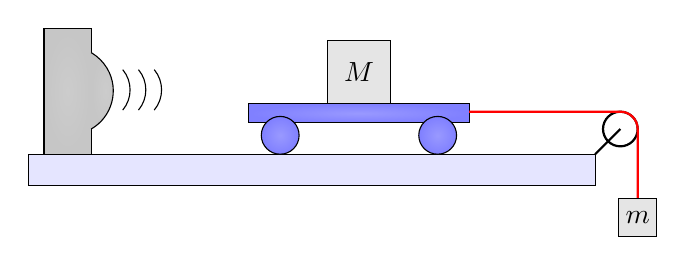
\begin{tikzpicture}
[scale = 8,
 plane/.style={draw=black,fill=blue!10},
 emit/.style={draw = black, inner color=lightgray!80 ,outer color=lightgray!90},
 cart/.style = {draw = black, inner color=blue!40,outer color=blue!50},
 mass/.style = {draw = black, fill = gray!20}
 ]
\draw [plane] (0.1,0) -- (1,0) -- (1,-0.05) -- (0.1,-0.05) -- (0.1,0);
\draw [emit] (0.125,0) rectangle (0.2,0.2);
\draw [emit] (0.2,0.04) arc (-60:60:0.07);
\draw (0.25,0.07) arc (-40:40:0.05);
\draw (0.3,0.07) arc (-40:40:0.05);
\draw (0.275,0.07) arc (-40:40:0.05);
\draw [cart] (0.45,0.05) rectangle ++ (0.35,0.03);
\draw [cart] (0.5,0.03) circle (0.03);
\draw [cart] (0.75,0.03) circle (0.03);
\draw [mass] (0.575,0.08) rectangle ++ (0.1,0.1) node[pos=.5] {\(M\)};
\draw [thick] (1.04,0.04) circle (0.0275);
\draw [thick] (1,0) -- (1.04,0.04);
\draw [red,thick] (0.8,0.0675) -- (1.04,0.0675) -- (1.04,0.0675) arc (90:0:0.0275) -- (1.0675,-0.1);
\draw [mass] (1.0675-0.03,-0.1-0.03) rectangle ++ (0.06,0.06) node[pos=.5] {\(m\)};
\end{tikzpicture}
\caption{The mass of \(m\) causes the cart and \(M\) to accelerate. }
\end{figure}

In order to avoid the movement of the cart prior to collection of data, the cart is held back by hand. Once collection of data has begun, the cart is allowed to move forward, and due to the weight of the mass \(m\), the cart begins to accelerate. Once the cart reaches a point close to the edge of the table, the cart is stopped and data collection ends.

Once the position data has been recorded, its first derivative with respect to time is taken numerically. This represents the velocity of the cart at a given time. The portion of time in which the velocity appears to be linear is the portion of time during which the cart is accelerating due to the weight of \(m\). The slope of this is recorded and deemed to be the acceleration experienced by the system during the time of interest.

In order to verify the relation described in Newton's second law of motion, two separate experiments are carried out. In the first, the total mass of the system is kept constant, but the forced applied to the cart is increased by moving mass from the top of the cart to the free hanging portion. While in the second, the force applied is kept constant and the total mass of the system is varied by changing the mass \(M\) on top of the cart.

\section{Data}
\subsection{Constant Mass, Changing Force}
The first experiment aimed to find the relationship between force and acceleration. The total mass of the system was kept constant at 350 g on top of the mass of the cart and string. That is to say that the sum of \(M\) and \(m\) was fixed to that value. However, the force was varied by allowing mass to move from \(M\) to \(m\) in different trials, increasing the force due to gravity acting on the cart.
\begin{table}[h]
	\centering
	\caption{Acceleration Measured given Constant Mass and Varying Force}
\begin{tabular}{|c|c|c|c|}
\hline
\(M\) (g) & \(m\) (g) & Force on Cart (N) & Acceleration (m/s\textsuperscript{2})
\\
\(\pm\) 0.1 & \(\pm\) 0.1  & &\\
\hline
300.0 & 50.0 & .490 \( \pm  \) 0.001 & 0.393 \(\pm\) 0.0025 \\
250.0 & 100.0 & .980 \( \pm  \) 0.001 & 0.769 \(\pm\) 0.01 \\
200.0 & 150.0 & 1.47 \( \pm  \) 0.001 & 1.272 \(\pm\) 0.008 \\
150.0 & 200.0 & 1.96 \( \pm  \) 0.001 & 1.781 \(\pm\) 0.005 \\
100.0 & 250.0 & 2.45 \( \pm  \) 0.001 & 2.246 \(\pm\) 0.004 \\
50.0 & 300.0 & 2.94 \( \pm  \) 0.001 & 2.723 \(\pm\) 0.007 \\
 
 \hline
\end{tabular}
\end{table}
\subsection{Constant Force, Changing Mass}
The second experiment aimed to relate mass and acceleration. The mass dangling of the edge of the table \(m\) remained constant and therefore the force felt due to gravity remained constant at \(m g\) as well. However, the mass \(M\) on top of the cart was allowed to vary.
\begin{table}[h]
	\centering
	\caption{Acceleration Measured given Constant Force and Varying Mass}
	\begin{tabular}{|c|c|c|c|}
		\hline
		\(M\) (g) & \(m\) (g) & Force on Cart (N) & Acceleration (m/s\textsuperscript{2})
		\\
		\(\pm\) 0.1 & \(\pm\) 0.1  & &\\
		\hline
		0.0 & 200.0 & 1.96  \(\pm\) 0.001 & 2.096 \(\pm\) 0.018 \\
		50.0 & 200.0 & 1.96 \(\pm\) 0.001 & 1.974 \(\pm\) 0.003 \\
		100.0 & 200.0 & 1.96 \(\pm\) 0.001 & 1.876 \(\pm\) 0.003 \\
		150.0 & 200.0 & 1.96 \(\pm\) 0.001 & 1.771 \(\pm\) 0.006 \\
		200.0 & 200.0 & 1.96 \(\pm\) 0.001 & 1.708 \(\pm\) 0.005 \\
		250.0 & 200.0 & 1.96 \(\pm\) 0.001 & 1.627 \(\pm\) 0.005 \\
		300.0 & 200.0 & 1.96 \(\pm\) 0.001 & 1.561 \(\pm\) 0.004 \\
		350.0 & 200.0 & 1.96 \(\pm\) 0.001 & 1.488 \(\pm\) 0.003 \\
		500.0 & 200.0 & 1.96 \(\pm\) 0.001 & 1.322 \(\pm\) 0.004 \\
		1000.0 & 200.0 & 1.96 \(\pm\) 0.001 & 0.976 \(\pm\) 0.005 \\
		
		\hline
	\end{tabular}
\end{table}
\\
\section{Analysis}
\subsection{Constant Mass, Changing Force}
If equation \eqref{EQ:1}, \( \vec{a} \propto  \vec{F} \), is true one would expect the acceleration of the cart to increase linearly as the force acting on the cart increases. Moreover, one would expect the slope of this line to be the reciprocal of the mass of the body being accelerated. This is more readily apparent if one chooses to write the expression in this form: \( a = \frac{1}{M_{tot}}F\) where \(M_{tot}\) is the mass of the whole system: cart, string, mass \(M\), and mass \(m\). 
\begin{figure}[h]
	\centering
	\caption{Acceleration as a Function of Force with a Constant Mass}
	\label{FIG:1}
	\begin{tikzpicture}
	\begin{axis}[%
	scatter/classes={%
		a={draw=black}},xlabel=Force on Cart (N),ylabel=Acceleration (m/s\textsuperscript{2})]
	\addplot[scatter,only marks,%
	scatter src=explicit symbolic]%
	table[meta=label] {
		x y label
		.49 0.393 a
		.98 0.769 a
		1.47 1.272 a
		1.96 1.781 a
		2.45 2.246 a
		2.95 2.723 a
	};
	\end{axis}
	\end{tikzpicture}
\end{figure}
Plotting these values, one sees what one might expect. In Figure 2 one sees the direct proportionality rather clearly, as the force on the cart increases its acceleration increases as well. One may try to fit a line of the form \( y = ax\) onto the data set, and if one does, ones finds an \(a\) value of  \( 0.9069 \pm 0.0015\) kg. If we recall that the slope a should have been \(1 / M_{tot}\), we can compute the total mass of the system. However, one must be wary of the uncertainty in the values. One may state that 
\begin{equation}
M_{tot} = \frac{1}{a},
\end{equation}
and therefore
\begin{equation}
\frac{\mathrm{d}M_{tot}}{\mathrm{d}a} = -\frac{1}{a^2}.
\end{equation}
One may use this to estimate the error in \(M_{tot}\)
\begin{equation}
\delta_{M_{tot}} = \left| \delta_a \frac{\mathrm{d}M_{tot}}{\mathrm{d}a} \right|
\end{equation}
Substituting in the expression and simplifying one may quantify the error as
\begin{equation}
\delta_{M_{tot}} =  \frac{\delta_a}{a^2}
\end{equation}
If we recall that \(M_{tot} = 1 / a\) then we may simplify further to
\begin{equation}
\delta_{M_{tot}} =  M_{tot} \frac{\delta_a}{a}
\end{equation}
or alternatively
\begin{equation}
\frac{\delta_{M_{tot}}}{M_{tot}} =  \frac{\delta_a}{a}
\end{equation}
Finally, if one choose to calculate \(M_{tot}\), the total mass of the system, one finds it to be \(1.103  \pm 0.0018\) kg. This means that the cart, string, and masses \(M\) and \(m\) should weigh \(1.103  \pm 0.0018\) kg.
\subsection{Constant Mass, Changing Force}
Alternatively, if one chooses to keep the force acting on the system constant but change the mass of the system one would expect the relationship to be \(a \propto 1 / M_{tot}\). Note that each \(M_{tot }\) was computed by summing the masses of \(M\), \(m\), and the cart and string. The cart and string together were measured to be \(0.5860 \pm 0.0005 \)kg. This time, one would expect the proportionality constant to be the force acting on the cart. This is made clear if one represents the acceleration in the form \(a = F \frac{1}{M_{tot}}\). The data collected support this notion, the graph in Figure 3 clearly shows an inverse relation between the total mass of the system and the acceleration undergone by the cart.
\begin{figure}[h]
	\centering
	\caption{Acceleration as a Function of Mass with a Constant Force}
	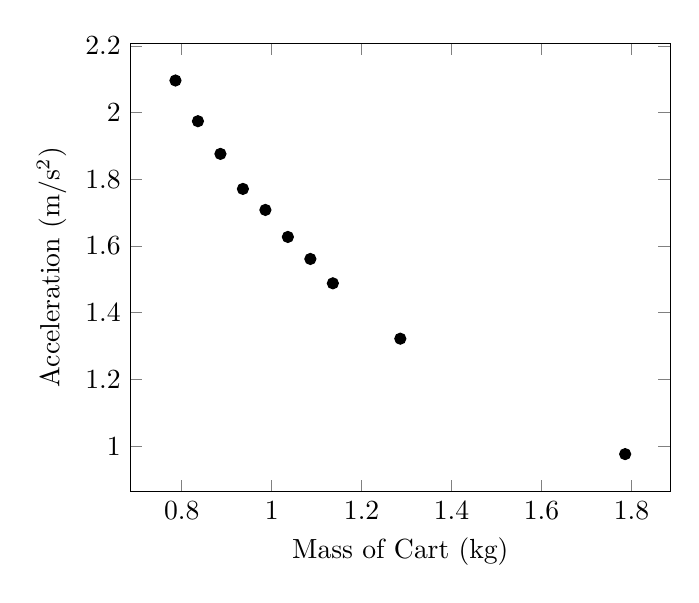
\begin{tikzpicture}
	\begin{axis}[%
	scatter/classes={%
		a={draw=black}},xlabel=Mass of Cart (kg),ylabel=Acceleration (m/s\textsuperscript{2})]
	\addplot[scatter,only marks,%
	scatter src=explicit symbolic]%
	table[meta=label] {
		x y label
		.786 2.096 a
		.836 1.974 a
		.886 1.876 a
		.936 1.771 a
		.986 1.708 a
		1.036 1.627 a
		1.086 1.561 a
		1.136 1.488 a
		1.286 1.322 a
		1.786 0.976 a
	};
	\end{axis}
	\end{tikzpicture}
\end{figure}

Again, one may fit a curve to this dataset.  This time the appropriate form is \(y = a/x \) where a is some constant. However, recall that in the context of the problem this may be written as \(a = F / M_{tot} \) where if is the constant that allows us to fit the curve. We can find this F to be \(1.672 \pm 0.009 \)N.
\section{Results and Conclusions}
All of the data collected supported Newton's Second law of motion. The relationship between acceleration and force is very clearly one of direct proportionality. In fact, the \(R^2\) value of the proportional fit was the incredibly high value of 0.994. The slope of this line was used to find the total mass of the system. This was found to be \(1.103  \pm 0.0018\) kg. This is an incredibly precise value, with the error bounds falling within 0.16 \% of the computed value. However, the measured value of the mass of the whole system is equal to \(0.936  \pm 0.005\) kg. This rather large inaccuracy manifests itself as a percent error of 17.8 \%.

The second experiment also supports Newton's second law. One can clearly see that the relationship between the acceleration and the mass of the accelerated body is one of inverse proportionality. Again, the fit of the inverse curve is incredibly tight, with an \(R^2\) value of 0.995. This time the force is calculated and found to be \(1.672 \pm 0.009 \)N. This also has very tight error bounds, accounting for only 0.5 \% of variation in the calculated force. But once again there is a high amount of inaccuracy. The force measured was \(1.96 \pm 0.001 \)N. This means there was a percent error of 14.6 \%.

Somewhere in the experiment an error of about 17\% is lurking. One might conjecture that friction was the cause of this consistent error. After all, not accounting for friction would cause one to conclude that either the car was heavier than it truly was or that the force acting upon it was smaller than it truly was, both of which were conclusions that the data would seem to support. However, in order for the error we see of 17 \% to occur the coefficient of rolling friction between the wheels and the table would have to be around 0.3. This value is much too large for wheels on a flat table, and therefore friction cannot truly be the main culprit. Also if one corrects for this amount of friction, the fit of the curves dramatically worsens which confirms that friction cannot have been the primary cause.

 Alternatively, one might think that perhaps the distance sensor was angled in some sense and therefore the distance measured was smaller than the true distance traveled by the car. Having done this, the cart would have appeared to moved slower, and therefore the mass would have been overestimated and force underestimated. However, in order for the difference to be so extreme as it is, the angle of the sensor would have had to have been around \ang{25}. An angle as large as \ang{25} would have been immediately noticeably and hence the angle cannot be the source of such a large error.
 
 Another possible explanation of this error involves the sensing of the distance traveled by the cart. The distance sensor collected distance data at 40 Hz, however the sensor was only rated to collect at 30 Hz. This may also have contributed to some sort of systematic error.
 
 Overall the 17\% error is likely a cause of a combination of theses factors and perhaps some others. However, the data are still in concordance the relationship described by Newton's second law of motion.
\end{document}